
%----------------------------------------------------------------------------------------
%	PACKAGES AND OTHER DOCUMENT CONFIGURATIONS
%----------------------------------------------------------------------------------------

\documentclass{article} % A4 paper size, default 11pt font size and oneside for equal margins
\usepackage[margin = 1in]{geometry}
\usepackage[portuguese]{babel}

\usepackage[utf8]{inputenc} % Required for inputting international characters
\usepackage[T1]{fontenc} % Output font encoding for international characters
\usepackage{fouriernc} % Use the New Century Schoolbook font
\usepackage{graphicx}

%----------------------------------------------------------------------------------------
%	TITLE PAGE
%----------------------------------------------------------------------------------------

\begin{document} 

\begin{titlepage} % Suppresses headers and footers on the title page

	\begin{figure}[t]
	\graphicspath{ {../../} }
	
\includegraphics[width = 8 cm]{logo.png}
	\centering
	\end{figure}
	
	\centering % Centre everything on the title page
	
	\scshape % Use small caps for all text on the title page
	
	\vspace*{\baselineskip} % White space at the top of the page
	
	%------------------------------------------------
	%	Title
	%------------------------------------------------
	
	\rule{\textwidth}{1.6pt}\vspace*{-\baselineskip}\vspace*{2pt} % Thick horizontal rule
	\rule{\textwidth}{0.4pt} % Thin horizontal rule
	
	\vspace{0.75\baselineskip} % Whitespace above the title
	
	{\LARGE 2\textsuperscript{\underline{o}} Projeto:\\Scheduling and Resource Sharing\par} % Title
	
	\vspace{0.75\baselineskip} % Whitespace below the title
	
	\rule{\textwidth}{0.4pt}\vspace*{-\baselineskip}\vspace{3.2pt} % Thin horizontal rule
	\rule{\textwidth}{1.6pt} % Thick horizontal rule
	
	\vspace{2\baselineskip} % Whitespace after the title block
	
	%------------------------------------------------
	%	Subtitle
	%------------------------------------------------
	
	 % Subtitle or further description
	Projeto de Sistemas Digitais \\ Docente: Paulo Flores

	\vspace*{3\baselineskip} % Whitespace under the subtitle
	
	%------------------------------------------------
	%	Editor(s)
	%------------------------------------------------
	
	
	\vspace{0.5\baselineskip} % Whitespace before the editors
	
	{\scshape\Large Afonso Rodrigues N\textsuperscript{\underline{o}} 67528 \\ Afonso Pereira N\textsuperscript{\underline{o}} 78949 \\ Miguel Rodrigues 
		N\textsuperscript{\underline{o}} 76176 \\} % Editor list
	
	\vspace{0.5\baselineskip} % Whitespace below the editor list
	
	\vfill % Whitespace between editor names and publisher logo
	
	\vspace{0.3\baselineskip} % Whitespace under the publisher logo
	
	08/11/2017 % Publication year

\end{titlepage}

\shipout\null %Blank Page without increasing page number 

%----------------------------------------------------------------------------------------

	
	\section{Introdução}
		Neste segundo projeto de laboratório são explorados os conceitos de gestão de recursos e calendarização, bem como o uso de memórias para receber dados e onde escrever dados.\\


		\noindent Com o conhecimento adquirido no laboratório anterior em relação ao funcionamento do software Vivado e à linguagem de descrição de hardware VHDL, é criado um programa que resolva uma iteração de um algoritmo (Método do Gradiente) para encontrar um mínimo local de uma equação polinomial de segundo grau. Os valores de cada variável (A, B, C, Xi e Step) estão presentes em memórias em posições consecutivas de memória, com 10 bits, as quais são acedidas sequencialmente de modo a realizar a primeira iteração de quatro conjuntos diferentes de dados. Cada iteração do algoritmo dá origem a três resultados a guardar (dy, Xn e y), originando um total de 12 valores de 40 bits a guardar. Estes são armazenados em posições sequenciais numa única memória de saída.\\	

		\noindent Considerando restrições de hardware, este projeto leva a que seja feita uma gestão e optimização dos recursos a utilizar que envolve calendarizar as operações a serem feitas, dando uso a diferentes recursos, como o \emph{ASAP Scheduling} ou a lista de prioridades.

	\section{Scheduling}
		Considerando apenas uma iteração do algoritmo completo, e admitindo que cada operação tem a duração de um ciclo de relógio, são obtidos os seguintes \emph{data flows} e lista de prioridades:

		\subsection{ASAP Scheduling}
			\emph{As Soon As Possible Scheduling}: Assim que seja possível realizar uma operação, esta é realizada, mesmo que o seu resultado só seja necessário muito tempo depois.


			\begin{figure}[ht]
				\begin{center}
					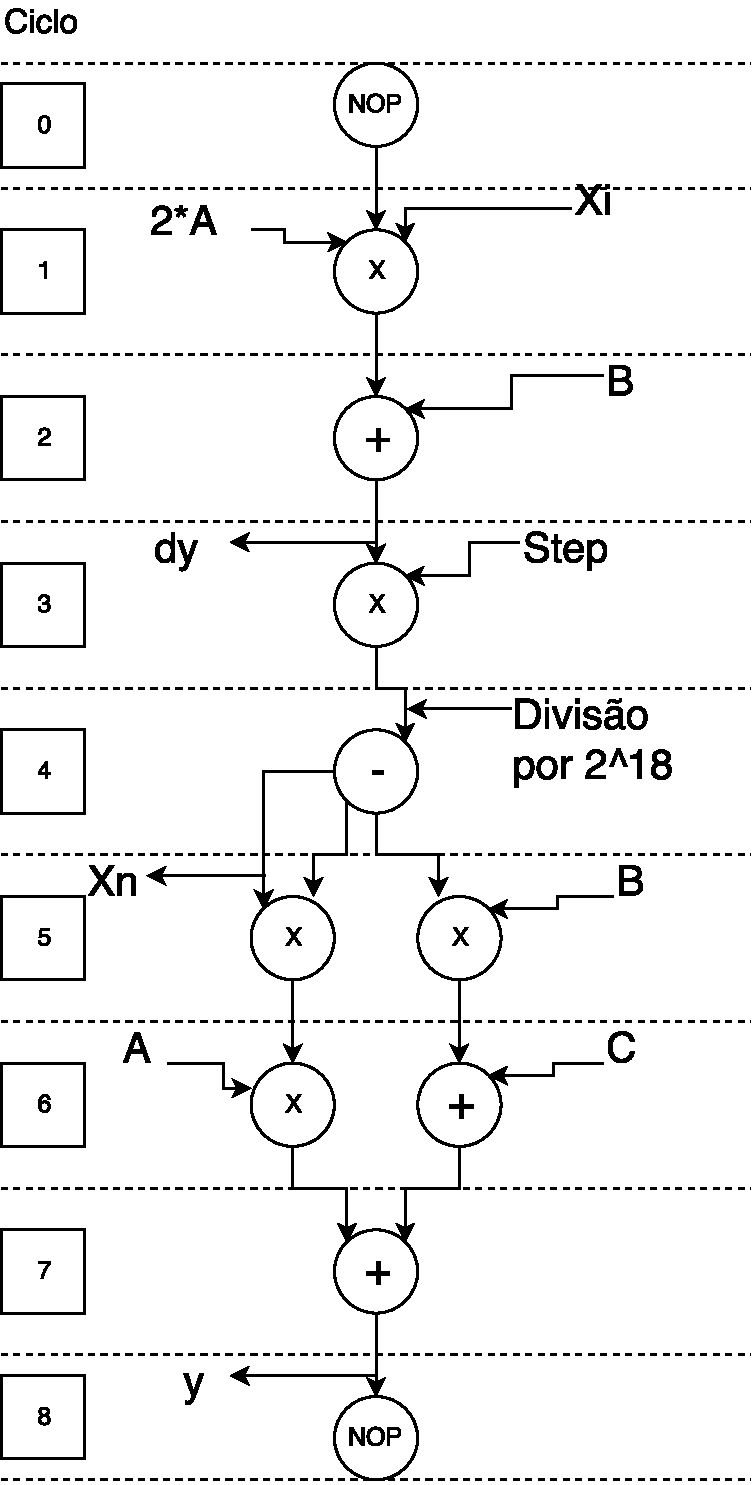
\includegraphics[width=1.5in]{ASAP.pdf}
					\caption{ASAP Scheduling}
					\label{fig:ASAP}
				\end{center}
			\end{figure}
			
			\textbf{Nota:} Tanto a multiplicação por 2 como a divisão por $2^{18}$ não requerem o uso de recursos adicionais, visto que são ambos múltiplos de 2, constituem apenas \emph{shifts} à esquerda (multiplicação) ou à direita (divisão). 

		\clearpage

		\subsection{ALAP Scheduling}
			\emph{As Late As Possible Scheduling}: As operações são realizadas o mais tarde possível sem afetar o número totald e ciclos de relógio (em comparação com o caso anterior), isto é, cada operação só se realiza no ciclo anterior a ser necessário o seu resultado.\\

			\noindent Neste projeto, este diagrama não vai ser diferente do presente na secção anterior, pois nenhuma operação pode ser realizada mais tarde sem atrasar toda a iteração (e nenhuma poderia ter sido feita mais cedo na secção anterior).

		\subsection{List Scheduling}
		
		A lista de prioridades usando o caminho crítico como métrica é a apresentada na Tabela~\ref{tab:Lsched}. Esta lista tem em conta que os recursos utilizados são os especificados: uma \emph{Arithmetic and Logic Unit} (com a sigla ALU na lista) e dois multiplicadores (com o símbolo X na lista).

		\begin{table}[htbp]
			\caption{List Scheduling}
			\begin{center}
				\begin{tabular}{|c||c||c|}
					\hline
					Nr & Operação & Prioridade \\
					\hline
					1 & X & 7 \\
					\hline
					2 & ALU & 6 \\
					\hline
					3 & X & 5 \\
					\hline
					4 & ALU & 4 \\
					\hline
					5 & X & 3 \\
					\hline
					6 & X & 3 \\
					\hline
					7 & X & 2 \\
					\hline
					8 & ALU & 2 \\
					\hline
					9 & ALU & 1 \\
					\hline
				\end{tabular}
			\end{center}
			\label{tab:Lsched}
		\end{table}

	\section{Circuito VHDl}
		\subsection{Unidade de Controlo}
			FSM, recursos, diagrama de estados talvez

		\subsection{Datapath}
			descrição datapath, o que faz, como faz, que recursos usa etc

		\subsection{Diagrama de Blocos, Recursos e Especificações}
		O diagrama de blocos presente na Figura~\ref{fig:Diagrama} descreve visualmente como funciona o datapath, recebendo os dados das memórias, o clk e o rst do circuito de topo e o oper do circuito de controlo. No entanto, recebe também outros sinais, como o valor dos contadores que vão decidir o endereço de memória onde escrever e o endereço onde ler.\\

		\noindent A área total deste circuito é constituída por 280 LUTs e 109 FFs. Quanto ao número de multiplexers, existem oito multiplexers a considerar, sendo que os restantes não são relevantes e são usados três registos no datapath, mas o número poderia ser reduzido para dois, pois a cada ciclo são gravados nos registos, no máximo, dois valores. Assim, olhando para a Figura~\ref{fig:ASAP}, as operações iniciais e as restantes do lado esquerdo poderiam estar gardadas em R1 e as duas do lado direito no registo R2, reduzindo o número de registos. No entanto, ter-se-ia de recorrer a diferentes multiplexers dos implementados.\\

		\begin{figure}[htbp]
			\begin{center}
				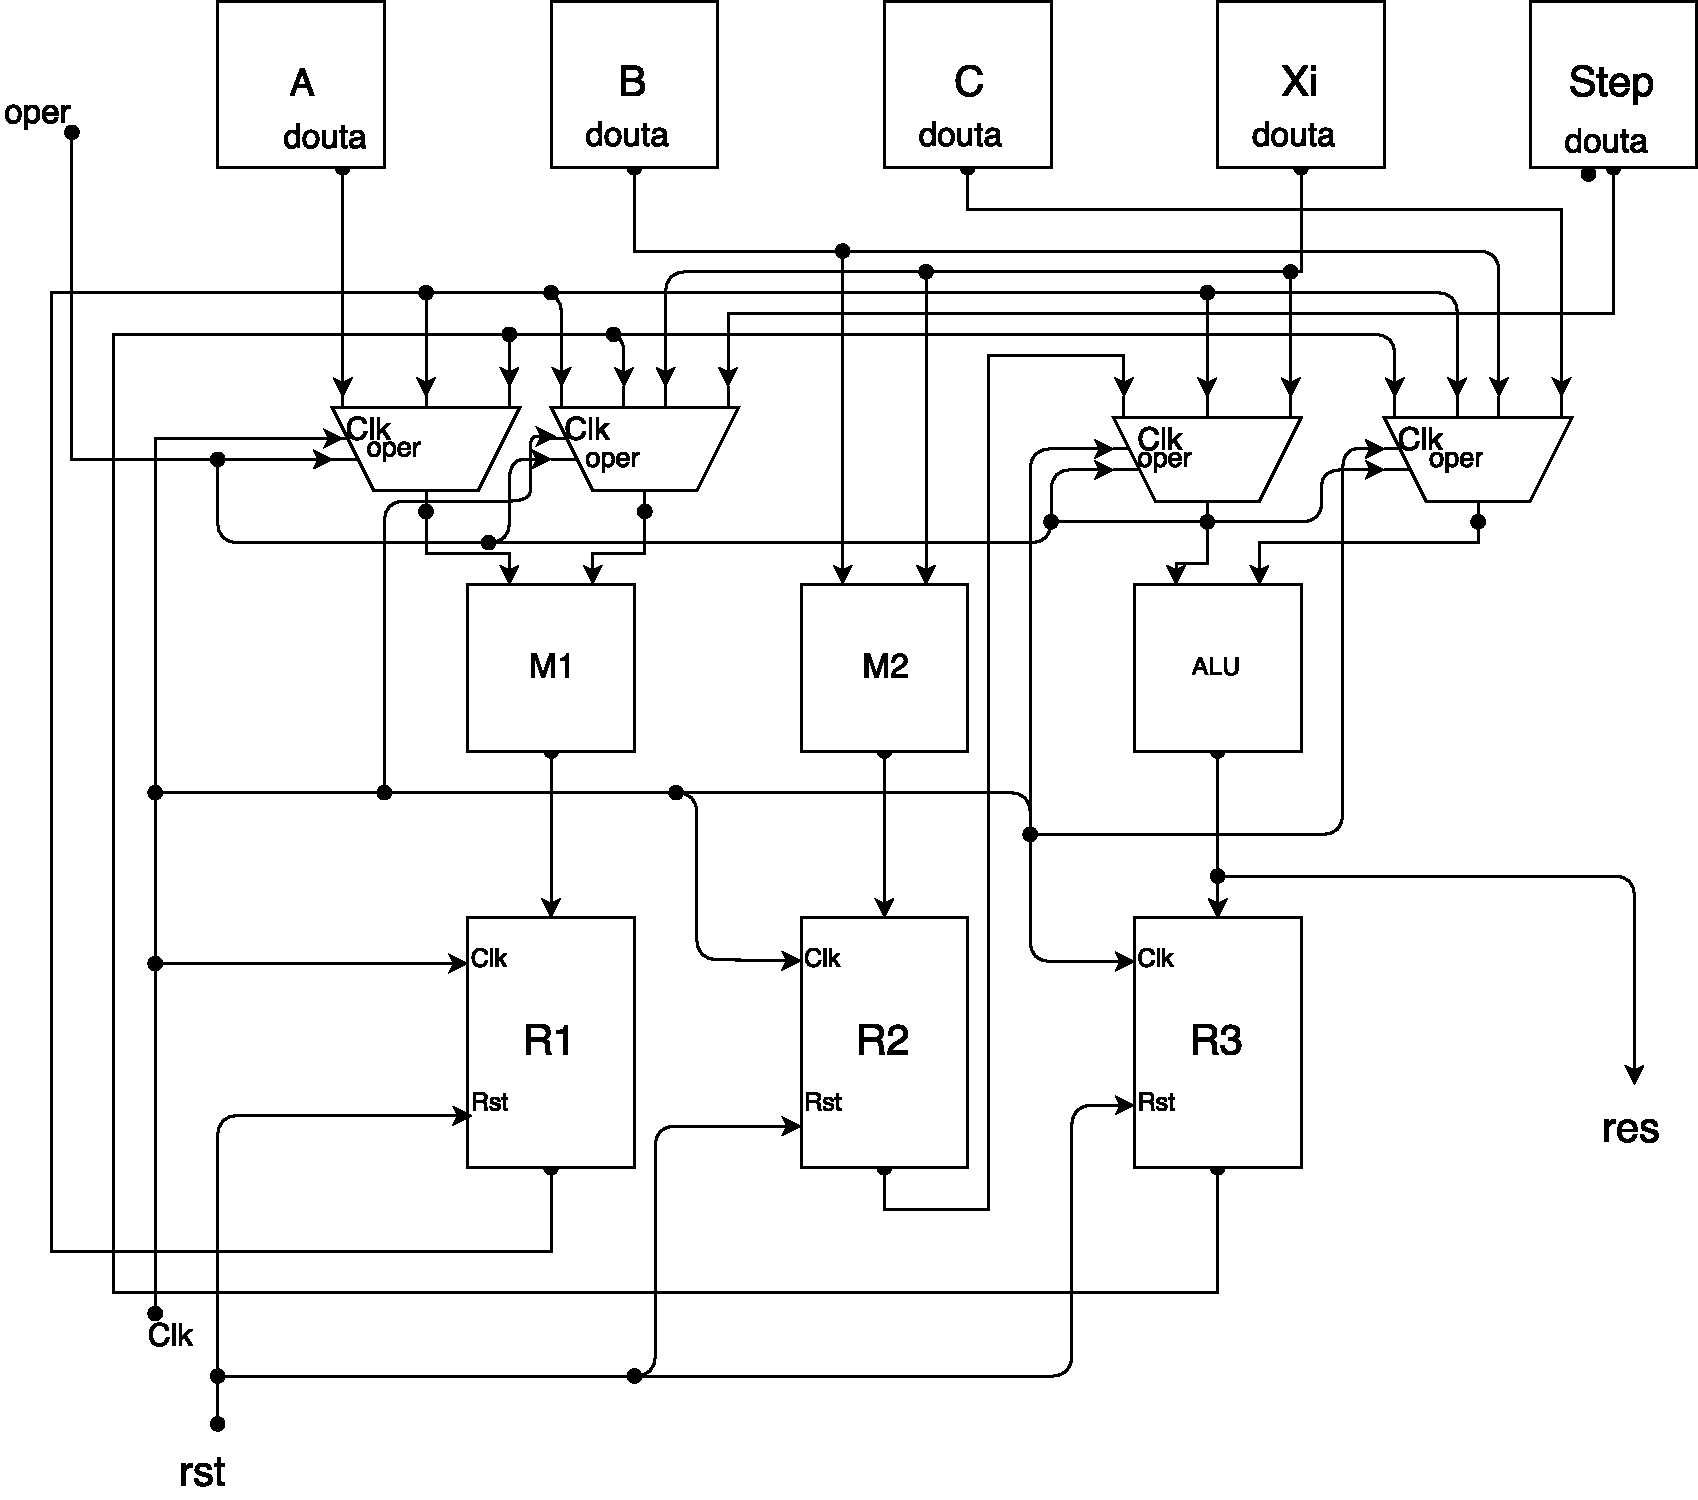
\includegraphics[width=4in]{Block.pdf}
				\caption{Diagrama de Blocos}
				\label{fig:Diagrama}
			\end{center}
		\end{figure}

		\noindent De acordo com os relatórios disponíveis após a síntese e implementação, com um período de clock de 11ns obtém-se um \emph{Total Negative Slack} de 0ns e um \emph{Worst Negative Slack} de 0.428ns, indicando um período adequado. No entanto, para que a \emph{Post-Implementation Timing Simulation} seja feita de forma correta, é necessário que o período a usar no \emph{testbench} seja de 15.0ns, originando uma frequência máxima de 66,(6) MHz. Nesta simulação é possível obter a latência do circuito, isto é, quanto tempo demora a iteração toda a ocorrer. Olhando para a Figura~\ref{fig:Sim}, feita com os dois primeiros conjuntos de valores disponibilizados e com os dois últimos e cujos resultados se apresentaram corretos, com recurso a cursores no momento em que é feito o reset e no momento em que o valor se torna realmente zero, infere-se que a latência é dada por 144.040 - 135.190 = 8.85ns.\\ 

		\begin{figure}[ht]
			\begin{center}
				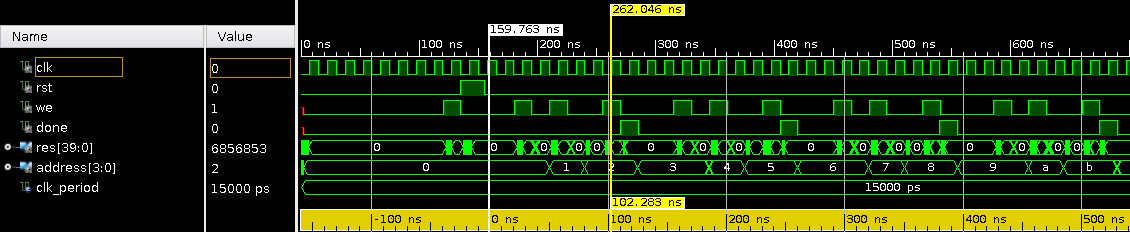
\includegraphics[width=6.5in]{sim.png}
				\caption{Simulação}
				\label{fig:Sim}
			\end{center}
		\end{figure}


	\section{Pipelining}

		Para melhorar a performance do circuito, é possível usar uma arquitetura de \emph{pipeline}, começando operações da iteração seguinte sem que a iteração atual esteja concluída. Sem utilizar recursos adicionais e admitindo que são usados apenas dois registos como referido na secção anterior, seria possível, apenas, encurtar um ciclo às restantes iterações após a primeira, pois como visto na Tabela~\ref{tab:Lsched}, é necessário o input de A até ao sexto ciclo, portanto a iteração seguinte só poderia começar no sétimo ciclo da iteração atual, onde se iria buscar o valor de A seguinte.\\

		\noindent No entanto, usando recursos adicionais é possível melhorar a performance do circuito.

	\section{Conclusão}

	
\end{document}
